
% 修論メインフォーマット
% 佐川さんの昨年の修論を借りています

\documentclass[a4j,12pt]{jreport}

% 修論フォーマットスタイルファイル
\usepackage{stylefile/mpaper}
\usepackage{stylefile/fancyheadings}
\usepackage{stylefile/cite}

% 追加パッケージ
\usepackage[dvipdfmx]{graphicx}
\usepackage{stylefile/multirow}
\usepackage{stylefile/slashbox}
\usepackage{url}
\usepackage{longtable}
\usepackage{epsfig}
\usepackage{comment}
\usepackage{algorithm}
\usepackage{algorithmic}
\usepackage{array}
\usepackage{booktabs}
\usepackage{comment}
\usepackage{here}
\usepackage{threeparttable}
\usepackage{subfig}

% 数式系パッケージ
\usepackage{amsmath}
\usepackage{amssymb}
\usepackage{bm}               % ベクトル表記(ボールド体)
\newcommand{\argmax}{\mathop{\rm arg~max}\limits}
\newcommand{\argmin}{\mathop{\rm arg~min}\limits}

\begin{document}

\begin{titlepage}
\thesis
{2019}                % 年度
{内視鏡画像からの\\簡易カルテ自動生成システム}       % 和文タイトル
{内藤 慎一郎}                % 氏名
{81821276}          % 学籍番号
{萩原 将文}         % 指導教員名
{2020}                % 卒業年
{3} % 卒業月
\end{titlepage}

% ------------------------------------ ヘッダ --------------------------------------

\renewcommand{\thepage}{--\roman{page}--}

% 和文アブスト
\jabstract
本論文では深層学習モデルを用いて内視鏡画像からの簡易カルテ作成を自動化する医師の支援システムを提案する。
従来の研究では(\ref{fig:overview})のように画像単位での学習と予測を行っており、患者単位での予測が不可能であった。
また一種類の病変のみの予測が可能なシステムであった。
本研究では(\ref{fig:overview})のように、病変が一つ以上存在するかのラベルと複数の病変ラベルから構成されるマルチラベルの教師データを用いた。
これによって患者単位での複数の病変の予測が可能なシステムとなった。
また既存研究では全ての画像に手動でラベルデータを付与していたのに対し、本研究では、マルチラベルデータを医師が実際に作成した簡易カルテから自動で生成した。
この学習データを用いて二次元と三次元の畳み込みニューラルネットワークをそれぞれ複数モデルずつ訓練し比較した。そしていくつかのモデルで高い推論性能を記録した。
また推論時の予測ラベルの生成において、複数の信頼度を持つ予測を生成することで、医師の判断の支援を行う機能も実装した。


\eabstract{} % 英文タイトル
% 英語アブスト
In this thesis, we devised an automatic creation support system for a draft of medical charts from endoscopic images using a deep learning model.
Inspection images of patients include many images without lesions even when a patient has lesions.
In the previous studies, learning and prediction were performed on an image basis, and prediction on a patient basis was difficult.
In this study, we created a system that can learn and predict multiple images in endoscopy on a patient basis.
This system is composed of datasets in which the information of a simple medical chart is summarized for each patient, and models that can learn images and datasets on a patient basis.
The system in the previous study could predict only one type of lesion.
In this study, label data consisting of a label indicating whether one or more lesions exist and a plurality of lesion labels is used.
These improvements make it possible to predict multiple lesions on a patient basis.
In addition, in the existing study, label data was manually assigned to all images, whereas in this study, multi-label data is automatically generated from a simple chart actually created by a doctor.
Using this learning data, we trained and compared several models of 2D and 3D convolutional neural networks. 
Some models recorded high inference performance for the task of predicting 10 or more multi-label simultaneously.
The F1-Score is 98\% or more in determining whether a patient had a lesion, and the F1-Score is 50\% or more in predicting multiple lesion information.
We also generate predictions with multiple reliability levels when predicting labels.
In the prediction of multiple lesion information, the precision is 87\% or more for highly reliable predictions, and the recall is 81\% or more for lowly reliability predictions.
As a result, the proposed system can be used to support the judgment of doctors.


% 目次
\contents

\pagenumbering{arabic}

% ------------------------------------ 本編 --------------------------------------
\chapter{序論}
現在機械学習の分野において深層学習による画像処理\cite{CNN,AlexNet,VGG,ResNet}、系列データ処理\cite{RNN,GRU,LSTM,Transformer}が高い精度を記録している。
このため文字や画像や音声などの認識\cite{DL_LVCSR,ImageNet}や生成\cite{GAN,VAE}、翻訳\cite{Transformer,Seq2Seq,effective_attention}や検索\cite{anxious_learning}といった自然言語処理に幅広く用いられるようになっている。
また化合物の性質予測\cite{Chemistry1,Chemistry2}やゲノム構造の解析\cite{Genomics}、株価の予測\cite{stock_prediction1,stock_prediction2}のように、生物学や化学や経済学などの情報工学分野を超えた様々な分野においても用いられてきている。

この流れの中で医学分野においても様々な用途で深層学習が用いられてきている。
例としては皮膚画像による皮膚ガンメラノーマの判定\cite{skin_cancer_melanoma}や放射線画像による深層学習解析\cite{radiology}などがあげられる。

他にも医学分野において深層学習を用いた自動化によって診断の精度向上や作業の効率化が期待できる用途がある。
その中でも内視鏡画像の解析が挙げられる。
既存研究には、内視鏡画像による胃癌判定\cite{stomach_cancer}や食道癌\cite{esophageal_cancer}の判定がある。
これらの研究は内視鏡画像を一枚ずつラベル付けして学習したもので、内視鏡検査における画像のすべてを学習しているわけではない。
このためより効果的な用途として内視鏡画像からの簡易カルテの生成が挙げられる (図\ref{fig:overview})。
現在簡易カルテの生成は人手によって行われており、各患者ごとに数分の時間がかかっている。
さらに大量の2重チェックを行う必要がある。
したがって医師の貴重な時間の多くを簡易カルテ作成に費やさなければならないという大きな問題がある。
これらの作業が自動化されることによる医師の負担削減が大きく期待できる。
また病変見落としが医師によっては2割以上といったデータ\cite{medical_problem2}もある。
自動化により精度の高い予測が可能になると、病変の見落としなども減らすことが可能になる。

しかしながら深層学習を医学分野に用いることに関していくつかの問題がある。
一つ目は倫理的な問題である。
医療における診断という大きな責任を伴う判断において、深層学習のような機械学習モデルを用いることには責任の所在がなくなるという課題がある。
現在の深層学習モデルはブラックボックスであり、判断の根拠が不明となっている。
このため医療分野における責任ある判断をまかせることにはまだ至っていない。
二つ目はプライバシーの問題である。
患者の診断データや内視鏡画像は重要度の非常に高いプライバシーデータであり、実際の推論システムにおいて患者のデータが特定可能な形で出力されてしまうことを必ず避けなければならない。

本研究では簡易カルテという精密検査や診断の確定がなされる前の作業における支援システムとして導入する。
したがって最終的な判断の責任は医師にある。
また学習データの作成では、簡易カルテから学習データのマルチラベルを作成するに当たって、質的診断の項目を自動で収集してマルチラベル化するため、プライバシー情報が完全に学習データに含まれない。
学習においても、内視鏡画像とマルチラベルデータのみを深層学習モデルに通した。

\begin{figure}[htbp]
    \centering
        \subfloat[][従来手法 (Lesion A のみの予測)]{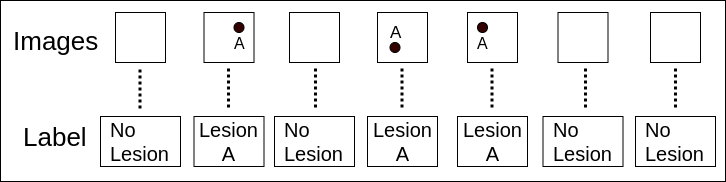
\includegraphics[width=100mm]{./fig/ieice0_0.png}\label{fig:overview0}} \quad
        \subfloat[][提案手法 (Lesion A, B,他多数,の予測)]{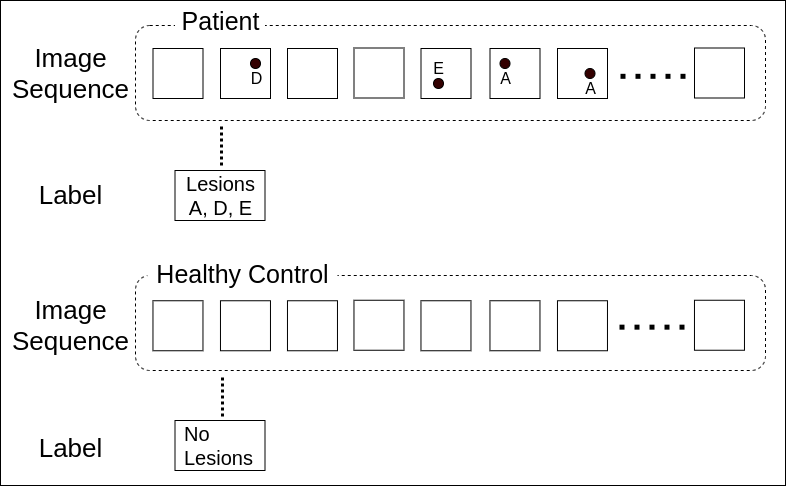
\includegraphics[width=100mm]{./fig/ieice0_1.png}\label{fig:overview1}} \quad
    \captionsetup{format=plain,font=normalsize,margin=30pt,name=図}
    \caption[]{全体概要}
    \label{fig:overview}
\end{figure}

既存研究では各患者に対して数十枚ある内視鏡画像すべてに手動で病名情報をラベリングしている。
したがって深層学習を用いるためには数十万の学習データを用意する必要があるために膨大な時間がかかっている。
全ての画像においてラベリングをした教師あり学習であるために高い精度を記録しているが、推論時も各画像単位で行われるため、画像を用いた診断として用いることはできるが簡易カルテの作成の自動化には至っていない。
なぜなら簡易カルテの作成の自動化には患者単位での予測が必要だからである。
このため本研究では医師が作成した簡易カルテに対して自然言語処理を行い、教師データとしてマルチラベルを作成した。
このマルチラベルデータは二つの部分から構成されている。
一番目のラベルは内視鏡画像の中に病変があるか否かを示す値が格納されており、二番目以降は頻出病名に対応した複数のラベルが並んでいる。
マルチラベルデータは簡易カルテの病名情報を要約したものとして用いることができる。
内視鏡画像とマルチラベルデータの関係性を直接学習させることによって、学習データの作成と学習全ての工程を自動化することに成功した。

学習手法に関しては、大きく分けて二つの手法で実験した。
一つ目の手法は各患者における数十枚の画像をそれぞれ一枚ずつ入力し、出力をマルチラベルから損失を計算し、モデルを学習するものである。
二つ目の手法では各患者の全ての時系列画像を三次元データとして用いてモデルを学習した。

本論文では作成した学習データを二つの手法においてそれぞれ複数の深層学習モデルで学習と推論を行い、結果を比較した。

以下、第2章で関連研究について述べ、第3章で提案手法について、第4章で評価実験、第5章で考察、第6章で結論を述べる。


\chapter{関連研究}
\section{関連研究}
深層学習モデルに内視鏡画像を学習させた研究として、食道部分の内視鏡画像から食道がんの有無を判定したものがある。この研究では画像を一枚ずつラベル付けし、これらをConvolutional Neural Network (CNN)を用いて学習した。384人の患者から得られた8428枚の画像を訓練データとし、47人の食道がん患者と50人の食道がんではない患者から得られた1118枚の画像をテストデータとした。用いたモデルはSingle Shot Multibox Detector (SSD)であり、これは16層のCNNで物体検出に特化したものである。この研究では食道がんの早期発見のために10mm以下の小さな病変を検知できるモデルの学習に特化した。その結果95\%という高い再現率を記録したが、適合率は40\%ほどとなっている。またこの研究では通常の内視鏡画像であるwhite-light image (WLI)と内視鏡機器に搭載されている狭帯域光観察によって病変を見やすくした画像であるnarrow-band imaging (NBI)をそれぞれ分けたものと包括的に扱ったものの3つの場合で比較している。この比較ではどの場合でも再現率は高いが適合率が低くなっている。

この研究の課題としては大きく3つのことが挙げられる。一つ目は各画像への手動でのラベリングである。これにより学習データの準備に非常に時間がかかる上に、データ拡張に対応できない。このモデルは診断の補助には利用できるが医師の作業効率化の支援にはなっていない。二つ目は一つ目とも関連するが、学習データが少ないことである。現在深層学習モデルの学習には数十万の画像を用いるのが一般的であるが、この研究では1万に満たないものであり、結果の適合率が非常に低いのはこの課題によるものでもあると考えられる。三つ目はSSDというモデルの選択である。SSDは16層という比較的浅いCNNモデルであるが、物体検出というタスクに特化することで高い精度を記録したものである。機械学習における物体検出とは景色のなかにある動物の検出といったタスクであり、内視鏡画像の中にあるわずかな病変を検出するような高難度なタスクとは異なっている。この研究での結果はこのモデルの選択に大きく影響を受けてしまっていると考えられる。このため用いるCNNのモデルはより深い特徴抽出ができる多層のモデルかつ、大きさの異なる複数の特徴の組み合わせを学習できる残差構造をもっているものが望ましいと考えられる。
本論文においては以上の3つの課題を解決することを目標とする。


\chapter{提案手法}
\section{内視鏡画像からの簡易カルテ自動生成システム}
提案手法をデータセットの作成、モデルの作成、モデルの学習、評価指標から説明する。
すべての実装コードは筆者のgithubのレポジトリ (https://github.com/shinn1r0\\/endoscopic\_images2karte)にある。実装には主にPythonを用い、深層学習フレームワークにはPytorchを使用した。またプライバシー情報のためデータセット作成の元となる内視鏡画像と簡易カルテのデータ、それらから生成したデータセットは提供しない。
\subsection{データセットの作成}
本研究では画像を個別にマルチラベルと関連付けで学習する手法と各患者ごとの全ての画像をまとめてマルチラベルと関連付けで学習する手法の二つの手法で実験を行ったため、データセットも二つ用意した。簡易カルテからのマルチラベル生成と各画像における処理は共通であるが、その後の処理はそれぞれの手法で異なっている。
\subsubsection{簡易カルテからのマルチラベル生成}

\begin{figure}[tb]
    \begin{center}
        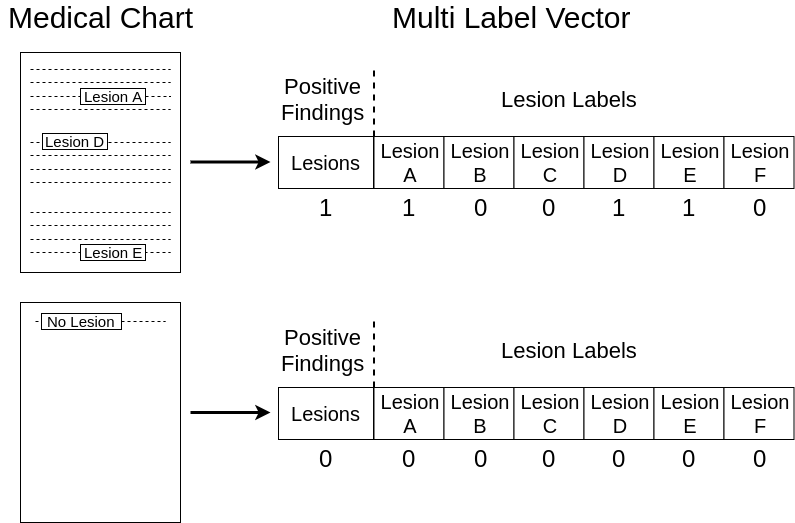
\includegraphics[width=75mm]{./fig/ieice1.png}
        \caption{Dataset Creation}
        \label{fig:multilabel}
    \end{center}
\end{figure}

簡易カルテからのマルチラベル生成 (図\ref{fig:multilabel})は以下の手順で行った。
\begin{enumerate}
    \item すべて異常なしの患者を抽出
    \item 簡易カルテ内の質的診断を言語処理
    \item 処理後の内容を全ての患者でまとめてカテゴリー化
    \item 頻出病名カテゴリー選択
    \item 各患者ごとにマルチラベル生成
    \item マルチラベルのone-hotベクトル化
\end{enumerate}
詳細を述べる。 (1)では簡易カルテ内の全ての行で異常なしとなっている患者を抜き出し、 (2)から (4)の処理には通していない。 (2)では簡易カルテ内の質的診断の項目のみを取り出し、言語処理を行った。この言語処理では文書であったり単語や数値の羅列であったりする質的診断をまず単語の系列データへと変換した。次にこれらを形態素解析や事前に用意した病名リストを用いた検索などを通して病名を表す単語とそれらに付随する情報を示す単語を抽出した。その際に複雑な付随情報を持つような病名は固有の処理を加えている。これにより簡易カルテの質的診断の項目では、各行が、先頭に病名単語があり、その後に付加情報単語が続く形式になった。 (3)では (2)の処理後の内容を全ての患者を通して集計し、同じ単語を同じラベル付けをして辞書に格納した。 (4)では辞書内で出現回数を計測し、指定した回数以上のラベルを頻出病名ラベルとして決定した。本研究ではすべて頻出病名を15個に設定した。 (5) (6)では各患者ごとにone-hot化したマルチラベルを生成した。マルチラベルは1番目のラベルには異常が一つでもある患者は1を、それ以外の患者は0が格納されている。これには (1)で抽出した情報を用いた。マルチラベルの2番目以降のラベルには頻出病名ラベルがある。 (2)から (4)で作成した情報を元に、各患者の質的診断の項目に頻出病名が存在する場合は1を、存在しない場合は0が格納されている。
\subsubsection{各画像における処理}
すべての画像は$256 \times 256$ピクセルにサイズ変更した。その後画像のRGBチャンネルそれぞれを正規化した。正規化のパラメータはRが平均0.485、標準偏差0.229、Gが平均0.456、標準偏差0.224、Bが平均0.406、標準偏差0.225に設定した。これらの値はすべて深層学習フレームワークのPytorchで推奨されている値を用いた。
\subsubsection{データセット分割}
2つの手法に合わせてデータセットを2つ用意した。それぞれのデータセットは訓練データ、検証データ、テストデータに分割した。
\begin{itemize}
    \item 画像を個別に入力する手法\\
この手法では、学習に用いる訓練データと検証データは画像を全患者に渡ってランダムにし、それぞれをマルチラベルと関連付けした。それに対して、テストでは患者単位での予測になるために、テストデータは患者単位で検査順に並んだ画像を系列データとしてマルチラベルと関連付けした。
    \item 画像を患者ごとにまとめて入力する手法\\
この手法では、学習とテストに用いる全てのデータを患者単位でまとめた。データは検査順に並べた画像を時間軸で連結させ、三次元データとし、それぞれマルチラベルと関連付けした。
\end{itemize}
\subsection{モデルの作成}
2つの手法に合わせてモデルも2つ用意した。どちらのモデルでも残差構造を持っていて、表現力の大きい多層のCNNを用いている。モデルの選択はPytorchで安定的に良い性能があるとされていて、用いられることが多いものを参考にした。
\begin{itemize}
    \item 画像を個別に入力する手法\\
この手法では残差構造 (Residential Connect)を持つCNN\cite{CNN}で最も一般的なResNet\cite{ResNet}を発展させたDenseNet\cite{DenseNet}を用いた。残差構造では、従来のネットワークでは同じ深さの層では同じ大きさの特徴しか抽出できなかったのに対して、ショートカットを用いることで同じ深さの層でも異なる大きさの特徴を抽出できるようになっている。ResNetはネットワークの主要部分で畳み込みを行って、ショートカット部分でその畳み込みを飛ばす構造をしている。DenseNetでは主要部分では畳み込みを行わず、分岐した部分に設置したDense Blockによって畳み込みを行い、その出力が主要部分で合流する構造をしている。これによりResNetより少ないパラメータ数で効率良く特徴抽出ができることが確認されている。
    \item 画像を患者ごとにまとめて入力する手法\\
この手法では画像を連結した三次元データを入力するため、CNNを三次元に拡張した3D-CNNを用いた。3D-CNNの中でも現在最も良い性能を持っている3D-ResNet\cite{3D_ResNet}を選択した。
\end{itemize}
\subsubsection{DenseNetのチューニング}

\begin{figure}[tb]
    \begin{center}
        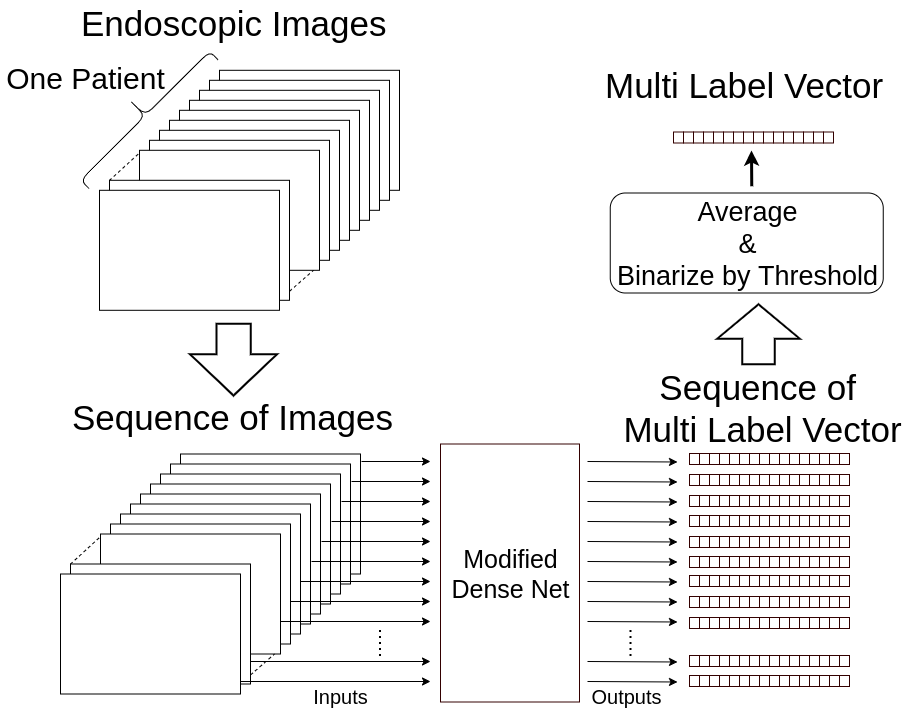
\includegraphics[width=75mm]{./fig/ieice2.png}
        \caption{DenseNet}
        \label{fig:densenet}
    \end{center}
\end{figure}

本研究に合わせてDenseNet (図\ref{fig:densenet})のチューニングをし、複数のモデルを用意した。全てのモデルにおいて共通していることは、特徴抽出部分をそのまま用いていることと、分類器部分の最終層のニューロン数をマルチラベルのクラス数と合わせていることである。これに加えて分類器部分を、通常の一層の全結合層のみの構造から、複数の全結合層とバッチ正規化とドロップアウトをからなる構造に変更したものも用意した。これはマルチラベル予測においては、抽出した特徴の組み合わせが1つのラベルの予測よりも複雑になるために、分類器においても深層の構造を用いて対応するためである。また今回の実験ではより複雑な特徴にも対応するために、層の数の異なる2つのDenseNetで学習した。それぞれDenseNet121\cite{DenseNet}とDenseNet161\cite{DenseNet}というモデルを用いた。このため合わせて4パターンで実験を行った。
\subsubsection{3D-ResNetのチューニング}

\begin{figure}[tb]
    \begin{center}
        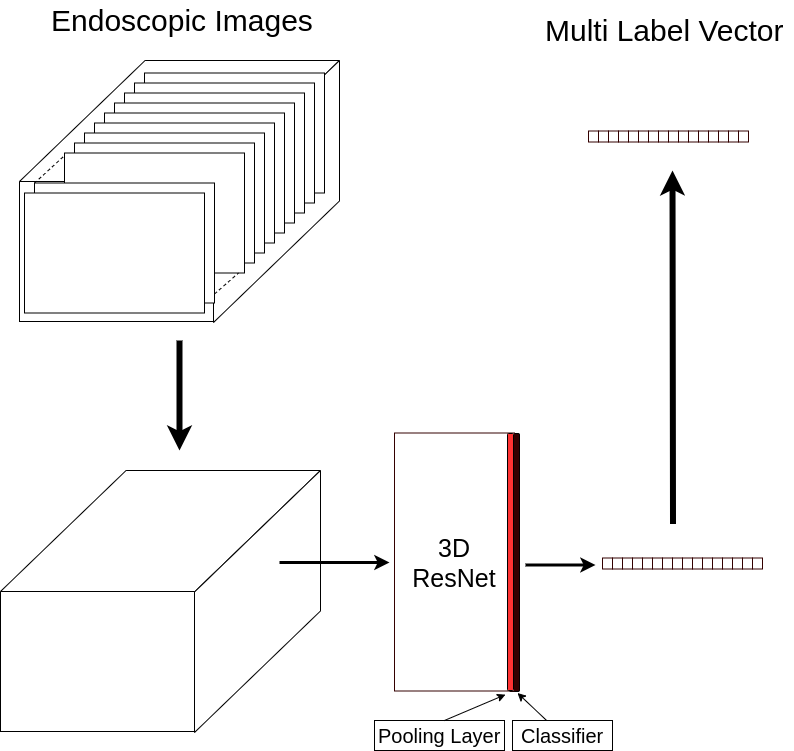
\includegraphics[width=75mm]{./fig/ieice3.png}
        \caption{3D-ResNet}
        \label{fig:3d_resnet}
    \end{center}
\end{figure}

本研究に合わせて3D-ResNet (図\ref{fig:3d_resnet})のチューニングをし、複数のモデルを用意した。特徴抽出部分の最終層において、通常では平均プーリングをして特徴を合算している。その際に特徴が損失する恐れがあったため、これを最大プーリングに置き換えたものも用意した。また分類器部分でもDenseNetのときと同じように、一層の全結合層のみのものと、複数の全結合層とバッチ正規化とドロップアウトをからなる構造に変更したものを用意した。このため合わせて4パターンで実験を行った。


\chapter{評価実験}
\section{評価実験}
\subsection{実験条件の設定}
\subsubsection{モデルの損失関数}
マルチラベル予測の学習のためバイナリ交差エントロピーを用いた。
\subsubsection{モデルの最適化手法}
確率的勾配降下法\cite{SGD}を拡張したAdaptive Moment Estimation (Adam)\cite{Adam}を使用した。これは勾配の大きさと更新量によって学習率を変化させていく方法で、様々なタスクで高性能を記録している。
\subsubsection{モデルの学習回数とバッチサイズ}
モデルの学習回数はすべて25にした。これは損失関数の推移から判断した。またバッチサイズはDenseNet121で50、DenseNet161で24、3D-ResNetで3とした。これは使用した計算機のメモリの容量によって決めた。
\subsection{評価指標}
評価指標は正解率、完全一致正解率、再現率、適合率、F1-Scoreの5つとした。
以下本文中の各データとは、画像を個別に入力する手法では各画像、画像を患者ごとにまとめて入力する手法では画像を時間軸で連結した3次元データを示す。
\subsubsection{正解率 (Acc)}
$各データにおける正解率 = \frac{正解したラベルの数}{マルチラベルにおける全てのラベルの数}$
を計算し、これをすべてのデータにおいて平均を計算した。
\subsubsection{完全一致正解率 (AllAcc)}
$AllAcc=\frac{マルチラベルにおける全てのラベルで一致したデータの数}{全てのデータの数}$
\subsubsection{適合率 (Precision)}
$Precision = \frac{真陽性}{真陽性+偽陽性}$

全てのデータにおける適合率を計算するために、各データにおける混合行列を集計し、その後適合率を計算した。
\subsubsection{再現率 (Recall)}
$Recall = \frac{真陽性}{真陽性+偽陰性}$

全てのデータにおける再現率を計算するために、各データにおける混合行列を集計し、その後再現率を計算した。
\subsubsection{F1-Score}
適合率と再現率がトレードオフの関係であるため、2つの指標を総合的に判断するためにF1-Scoreを用いた。

$F1{\rm \mathchar"712D}Score = \frac{Precision * Recall}{(Precision + Recall) / 2}$

\subsubsection{評価指標とモデルの性能の関係性}
\begin{itemize}
    \item 正解率\\
        正解率は指標としてモデルの性能をあまり評価できない。マルチラベル予測の際にこの指標を用いると、マルチラベルのクラス数が多いほど真陰性の割合が多くなり、実際の予測がほとんど行われていなくても高い数値が出るからである。
    \item 完全一致正解率\\
        完全一致正解率は指標としてモデルの性能をあまり評価できない。マルチラベル予測の際にこの指標を用いると、マルチラベルのクラス数が多いほど全てを一致させることが困難になり、ほぼ全てのクラスで正解しているもとと全く正解していないものを区別できない。
    \item 適合率\\
        適合率はマルチラベル予測の指標として一般的に用いられる。適合率は陽性であると予測したものの中で、実際に陽性であるものの割合である。これは本用途においては病変があると予測したものの中で、実際に病変があったものの割合となっており、誤検知の少なさの指標と言える。
    \item 再現率\\
        再現率はマルチラベル予測の指標として一般的に用いられる。再現率は実際に陽性であるものの中で、陽性であると予測できたものの割合である。これは本用途においては病変があるデータの中で、病変があると予測できたものの割合となっており、見落としの少なさの指標と言える。
    \item F1-Score\\
        F1-Scoreはモデルの性能を最も表していると言える。本実験ではこの数値が高いものを良いモデルとして評価する。
\end{itemize}

\subsection{DenseNetを用いた内視鏡画像からの\\マルチラベル予測}
\subsubsection{実験概要}
各画像をマルチラベルと関連付けしたデータセットを用いた。画像をモデルに入力し出力されたマルチラベルと教師データのマルチラベルから損失を計算し最適化を行った。モデルが出力したマルチラベルの各ラベルを二値化する際のしきい値を変化させた。その結果からテスト出力の際のしきい値を決定し、推論を行った。

\subsubsection{実験結果}
結果を以下に示す。
\begin{figure}[tb]
    \centering
        %\subfloat[][学習過程]{\includegraphics[width=70mm]{./fig/sample1.jpg}\label{fig:01}} \quad
        %\subfloat[][検証結果]{\includegraphics[width=70mm]{./fig/sample2.jpg}\label{fig:02}} \quad
        %\subfloat[][各しきい値におけるテスト]{\includegraphics[width=70mm]{./fig/sample3.jpg}\label{fig:03}} \quad
        %\subfloat[][推論結果]{\includegraphics[width=70mm]{./fig/sample4.jpg}\label{fig:04}} \quad
    \captionsetup{format=plain,font=large,margin=50pt,name=図}
    \caption[]{DenseNetを用いた内視鏡画像からのマルチラベル予測}
\end{figure}
\subsection{3D-ResNetを用いた内視鏡画像からのマルチラベル予測}
\subsubsection{実験概要}
各患者ごとに画像を時間軸で連結した三次元データとマルチラベルと関連付けしたデータセットを用いた。三次元データをモデルに入力し出力されたマルチラベルと教師データのマルチラベルから損失を計算し最適化を行った。モデルが出力したマルチラベルの各ラベルを二値化する際のしきい値を変化させた。その結果からテスト出力の際のしきい値を決定し、推論を行った。

\subsubsection{実験結果}
結果を以下に示す。
\begin{figure}[tb]
    \centering
        %\subfloat[][学習過程]{\includegraphics[width=70mm]{./fig/sample1.jpg}\label{fig:01}} \quad
        %\subfloat[][検証結果]{\includegraphics[width=70mm]{./fig/sample2.jpg}\label{fig:02}} \quad
        %\subfloat[][各しきい値におけるテスト]{\includegraphics[width=70mm]{./fig/sample3.jpg}\label{fig:03}} \quad
        %\subfloat[][推論結果]{\includegraphics[width=70mm]{./fig/sample4.jpg}\label{fig:04}} \quad
    \captionsetup{format=plain,font=large,margin=50pt,name=図}
    \caption[]{3D-ResNetを用いた内視鏡画像からのマルチラベル予測}
\end{figure}


\chapter{考察}
\section{考察}
\subsection{各実験における考察}
\subsubsection{DenseNetを用いた内視鏡画像からの\\マルチラベル予測における考察}
学習過程を見ると、損失がエポックが進むごとに減っていて、かつAccとAllAccの両方が上昇していることから、学習がきちんと進んでいることがわかる。また訓練損失が減少を続けているのに対して、検証損失が学習途中から上昇に転じている。これはデータに関して過学習を起こしているが、DenseNet121からDenseNet161に増やしたのに関わらず変化がないことから、これはモデルの大きさによって特徴表現が狭まっているわけではない。マルチラベル学習でバイナリ交差エントロピーを用いていることから、モデルの学習が進んで予測されるラベルが増えるに従って損失が増えやすくなっていると考えられる。また各画像をマルチラベルと関連付けて学習するこの手法では、病変がある患者において、病変が全く見られない部位の画像も病変の存在を示すマルチラベルと学習するために学習が安定しずらいと考えられる。しかしAccやF1-Scoreが良くなっていることから、学習は問題なく進んでいると見なすことができる。

検証結果を見ると、AllAccが30\%を超えていて、F1-Scoreも70\%を超えており、モデルがきちんと学習されていることがわかる。しかしこの結果には複数の問題がある。AllAccに関しては、マルチラベルの中でもそもそもラベルが真になっている部分の少ない教師データの際に予測ができているだけの可能性が高い。F1-Scoreもマルチラベルの一つ目の病変が1つでもあるかどうかのラベルの推論結果が良いために、全体の結果が良くなっていると考えられる。このためマルチラベルの検証結果を一つ目のラベルと二つ目以降のラベルに分離した結果を提示した。この結果を見ると、一つ目のラベルはPrecisionとRecallともに98\%を超えていて、病変があるかどうかの判定は高い精度を持っていることがわかる。また二つ目以降のラベルでもPrecisionが75\%、Recallが40\%、F1-Scoreが53\%と判定がある程度はできていることがわかる。

検証結果では推論時のマルチラベルの二値化の際のしきい値が0.5に設定されているが、テストの際にはしきち値を0.1から0.9まで0.1ずつ変化させてPrecisionとRecallの推移を見た。PrecisionとRecallの値の性質上、両者はトレードオフの関係にあり、しきち値が低いとRecallが上がり、高いとPrecisionが上がる。この実験の結果、しきち値が0.3のときに両者がバランス良く、F1-Scoreが一番高かった。またしきい値が0.1のときにRecallが81\%と一番高く、しきい値が0.6のときにPrecisionが87\%と一番高くなった。

この結果を用いて本研究での提案システムとしては、しきい値が0.6のときの結果を予測の範囲は狭いが信頼度の高い予測として、しきい値が0.1のときの結果を信頼度は低いが広範囲の予測として用いる。これにより、医師の診断時の判断の支援も行える。

\subsubsection{3D-ResNetを用いた内視鏡画像からの\\マルチラベル予測における考察}
3D-ResNetを用いた実験ではDenseNetでの場合と同様に、損失の推移やAccとAllAccの値から学習が問題なく行われていると見なすことができる。またDenseNetの場合とは異なり、学習回数が進んでも訓練損失と検証損失の差が開いておらず、過学習が抑えられていると。これは各患者ごとに画像を時間軸で連結した三次元データを用いていることから、全く関係ない特徴量とマルチラベルが学習されることが減り、学習が安定したことが考えられる。しかしAllAccやF1-ScoreがDenseNetと比べてわずかに低くなっている。これは3D-CNNを用いたことにより、特徴抽出部分の最終層での特徴の合算の際に特徴が多少消失してしまったためであると考えられる。

検証結果はDenseNetの場合と同様に、一つ目のラベルはPrecisionとRecallともに98\%を超えていて、病変があるかどうかの判定は高い精度を持っていることがわかる。また二つ目以降のラベルでもPrecisionが71\%、Recallが39\%、F1-Scoreが50\%と判定がある程度はできていることがわかる。しかし検証結果も学習過程での見られたのと同じ傾向があり、DenseNetよりもわずかに結果が低くなっている。

推論時のマルチラベルの二値化の際のしきい値の推移を見ると、しきい値が0.2のときにPrecisionとRecallのバランスが良く、F1-Scoreが一番高かった。またしきい値が0.1のときにRecallが83\%と一番高く、しきい値が0.9のときにPrecisionが88\%と一番高かった。しかし、しきい値が0.9のときはRecallが9\%、F1-Scoreも17\%と非常に低くなっている。このためしきい値が高すぎて予測ラベルが少なすぎる状態になっていると考えられるため、しきい値が0.7のときがPrecisionが75\%かつRecallが34\%と信頼度の高い予測として有用だとみなすことができる。これにより、その他の結果と同様に3D-ResNetのときはDenseNetのときよりも少し精度が低いという結果になった。

\subsection{全体における考察}
画像を個別に入力する手法と画像を患者ごとにまとめて入力する手法の両方で非常に有用な結果が出たと言える。画像を患者ごとにまとめて入力する手法のほうが、関係ない特徴とラベルの学習がなくなるために学習は安定する。それに対して画像を個別に入力する手法の方は、学習は不安定化する。しかし予測の際も1枚ずつ予測し、その結果を患者ごとに集約するために、間違った予測が弱まり、正しい予測が重ね合わさることで、患者単位の予測では高い精度を出すことに成功した。どちらの手法のモデルでもしきち値の変更でPrecisionが70\%前後の予測を信頼度の高い予測として、Recallが80\%前後の予測を信頼度は低いが可能性としてはありえる予測として提供することができ、診断の際の判断の支援と見逃しの防止の両方を満たすシステムとして利用することができる。


\chapter{結論}
\section{結論}
結論



% ------------------------------------ フッタ ----------------------------------------

% 謝辞
\acknowledgment
本研究を行うにあたり、指導教官の萩原将文教授から終始熱心なご指導を承りました。ここに感謝の意を表します。また研究室の方々には様々な相談をさせて頂き、特に同期の方々には研究を通じて活発な議論にお付き合い頂きましたことを感謝致します。さらに慶応義塾大学医学部消化器内科との共同研究であったため、種本俊先生と筋野智久先生には多大なご協力を頂き大変感謝いたします。


% 参考文献
\bibliographystyle{./stylefile/jcustom}
\bibliography{./reference/reference}

% ------------------------------------ 付録 ---------------------------------------
\appendix
\chapter{他のモデルにおける実験}
\section{実験\ref{sec:ex11}}
実験\ref{sec:ex1}の他のモデルにおける実験を行った。

\newpage
\subsection{モデル2の結果}
\begin{figure}[htbp]
    \begin{center}
        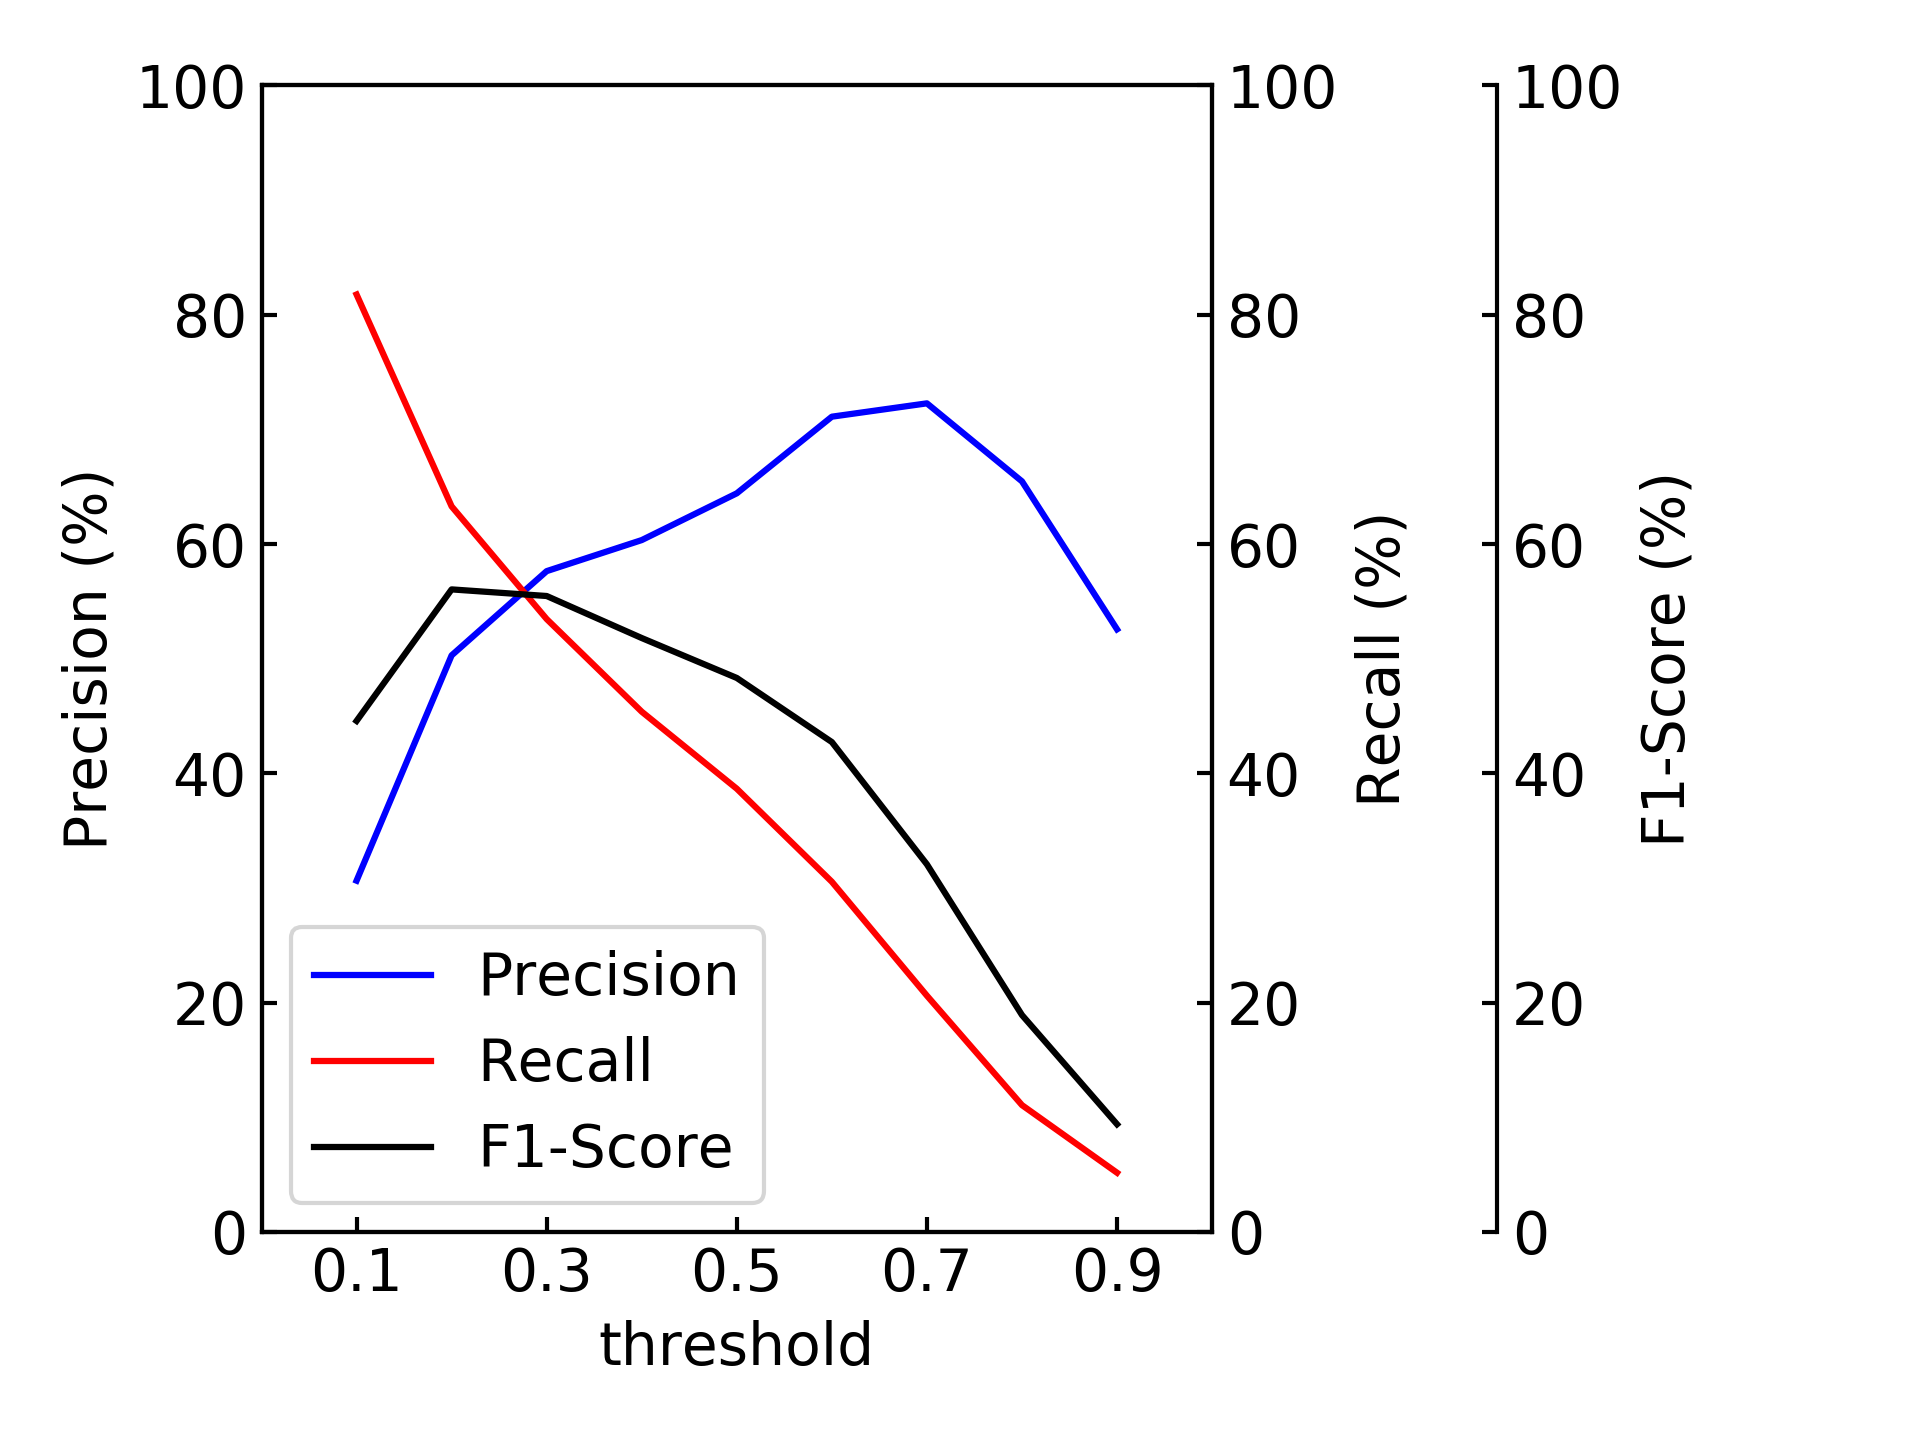
\includegraphics[width=150mm]{./fig/densenet121_e_p02threshold.png}
        \caption{しきい値を変化させた際の適合率と再現率の変化}
        \label{fig:densenet121_e_result_threshold}
    \end{center}
\end{figure}

\newpage
\subsection{モデル3の結果}
\begin{figure}[htbp]
    \begin{center}
        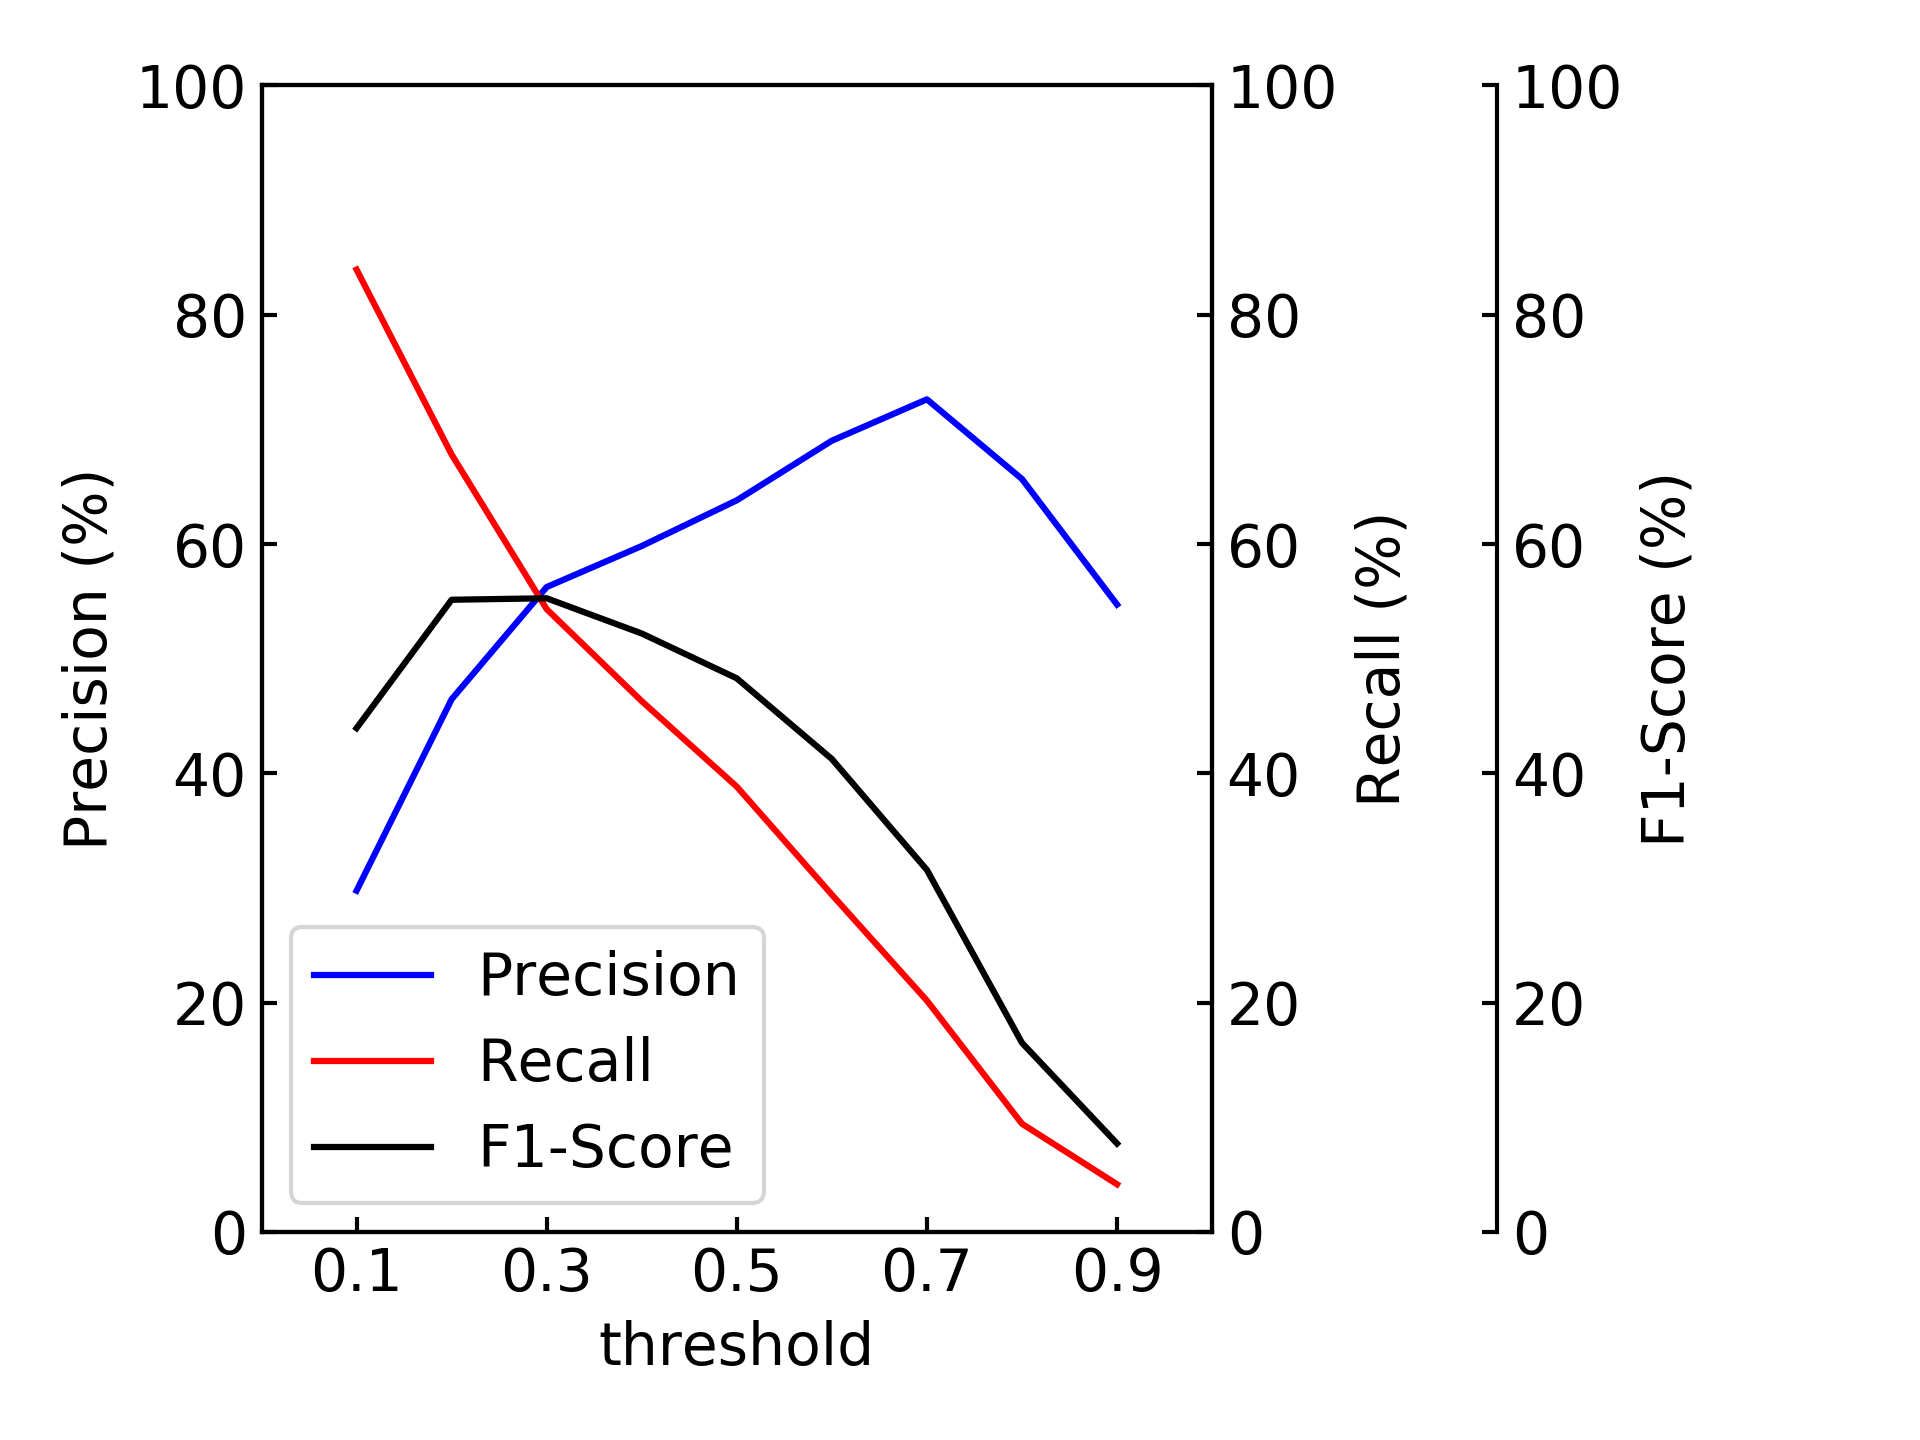
\includegraphics[width=150mm]{./fig/densenet161threshold.png}
        \caption{しきい値を変化させた際の適合率と再現率の変化}
        \label{fig:densenet161_result_threshold}
    \end{center}
\end{figure}

\newpage
\subsection{モデル4の結果}
\begin{figure}[htbp]
    \begin{center}
        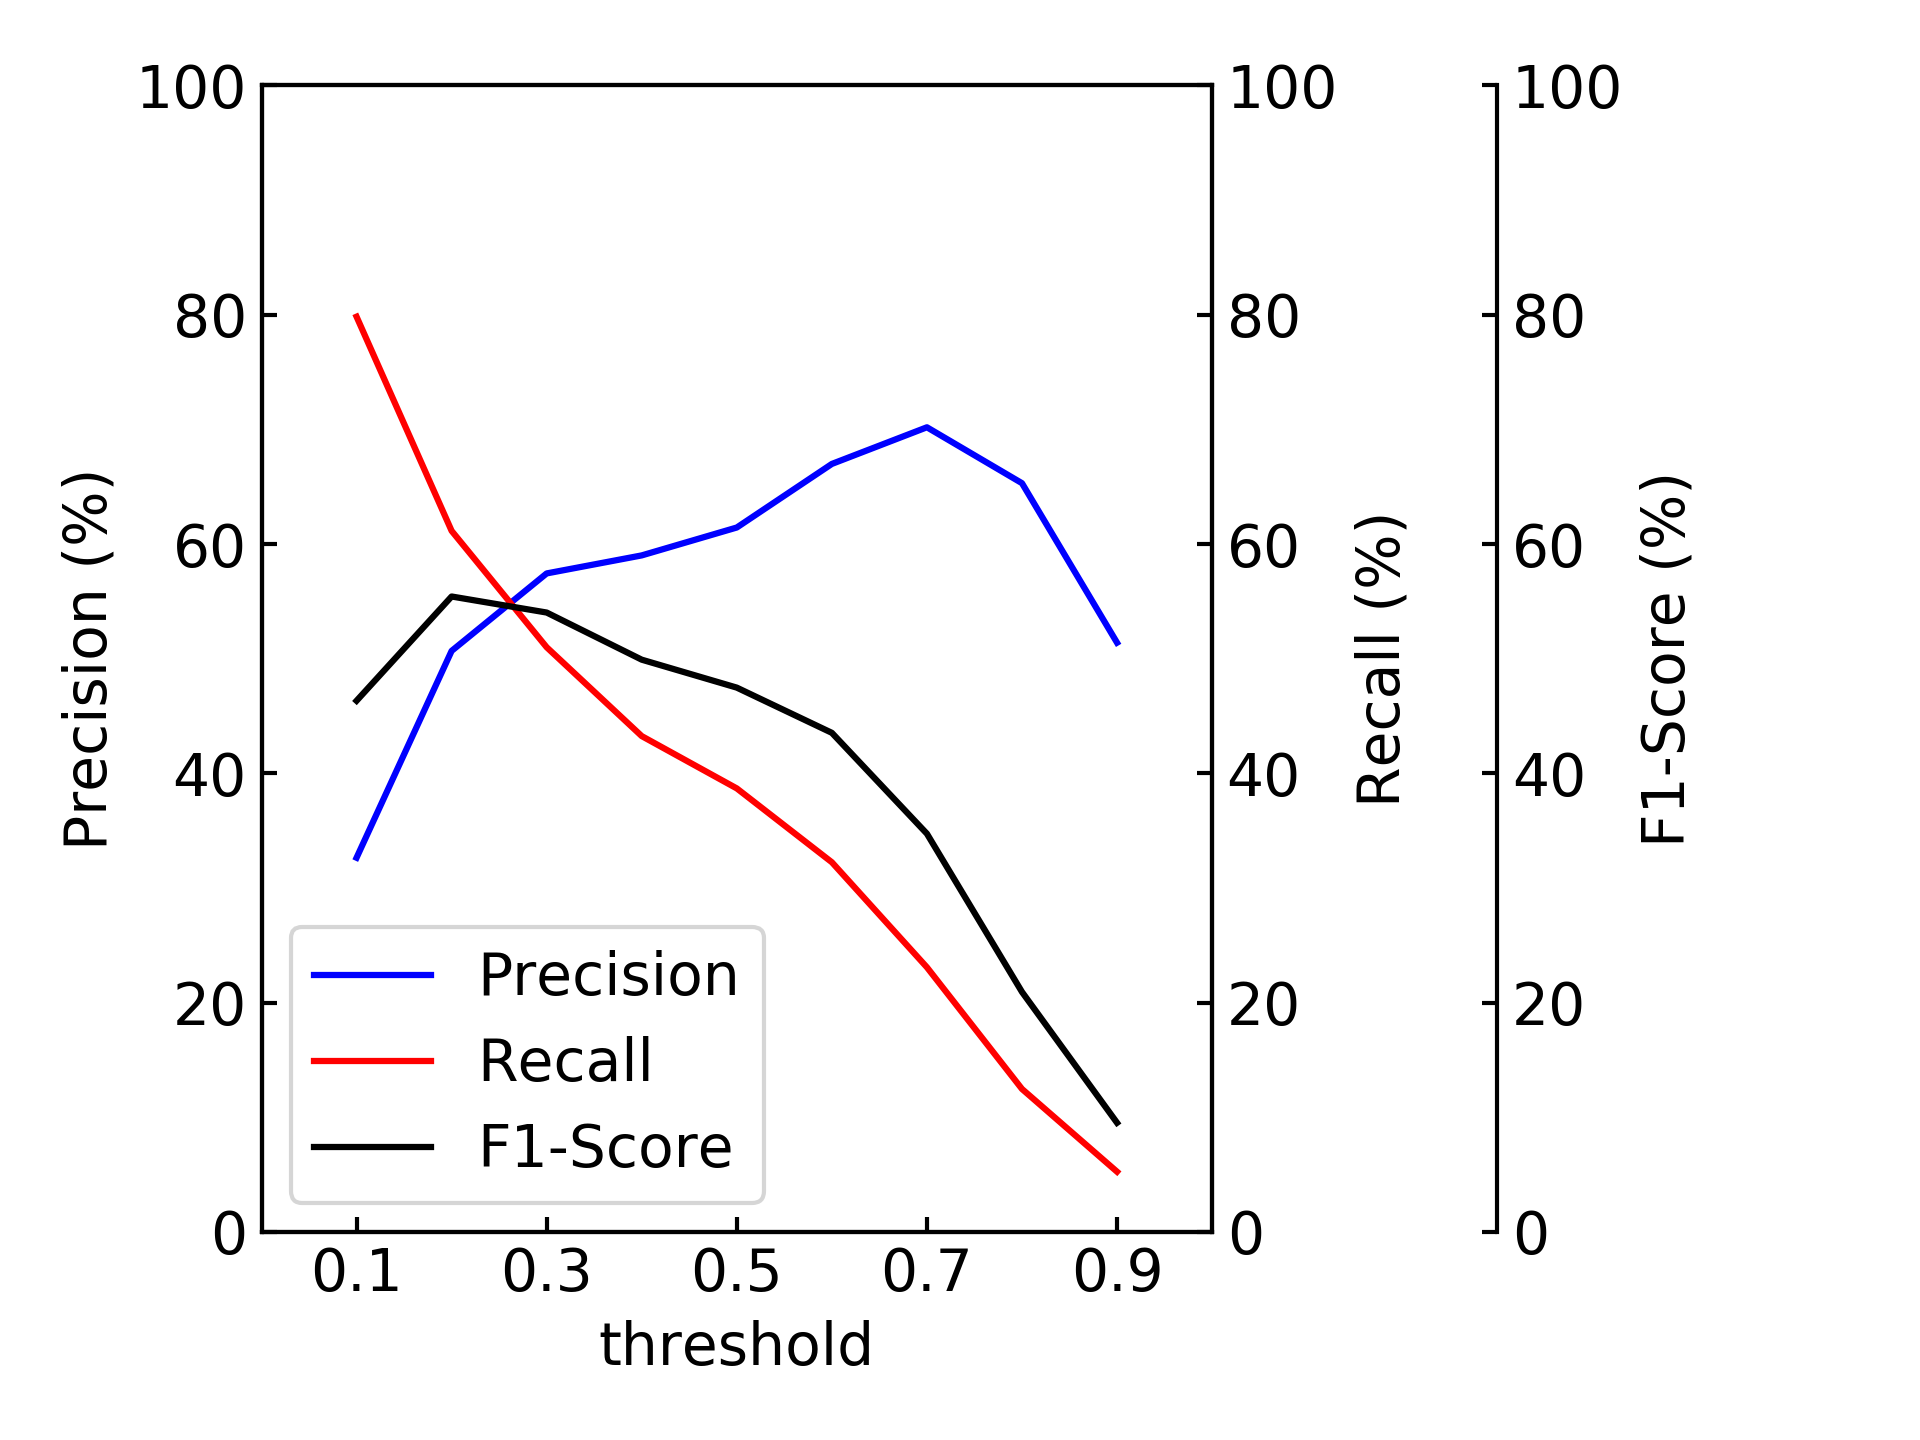
\includegraphics[width=150mm]{./fig/densenet161_ethreshold.png}
        \caption{しきい値を変化させた際の適合率と再現率の変化}
        \label{fig:densenet161_e_result_threshold}
    \end{center}
\end{figure}

\section{実験\ref{sec:ex22}}
実験\ref{sec:ex2}の他のモデルにおける実験を行った。

\newpage
\subsection{モデル2の結果}
\begin{figure}[htbp]
    \begin{center}
        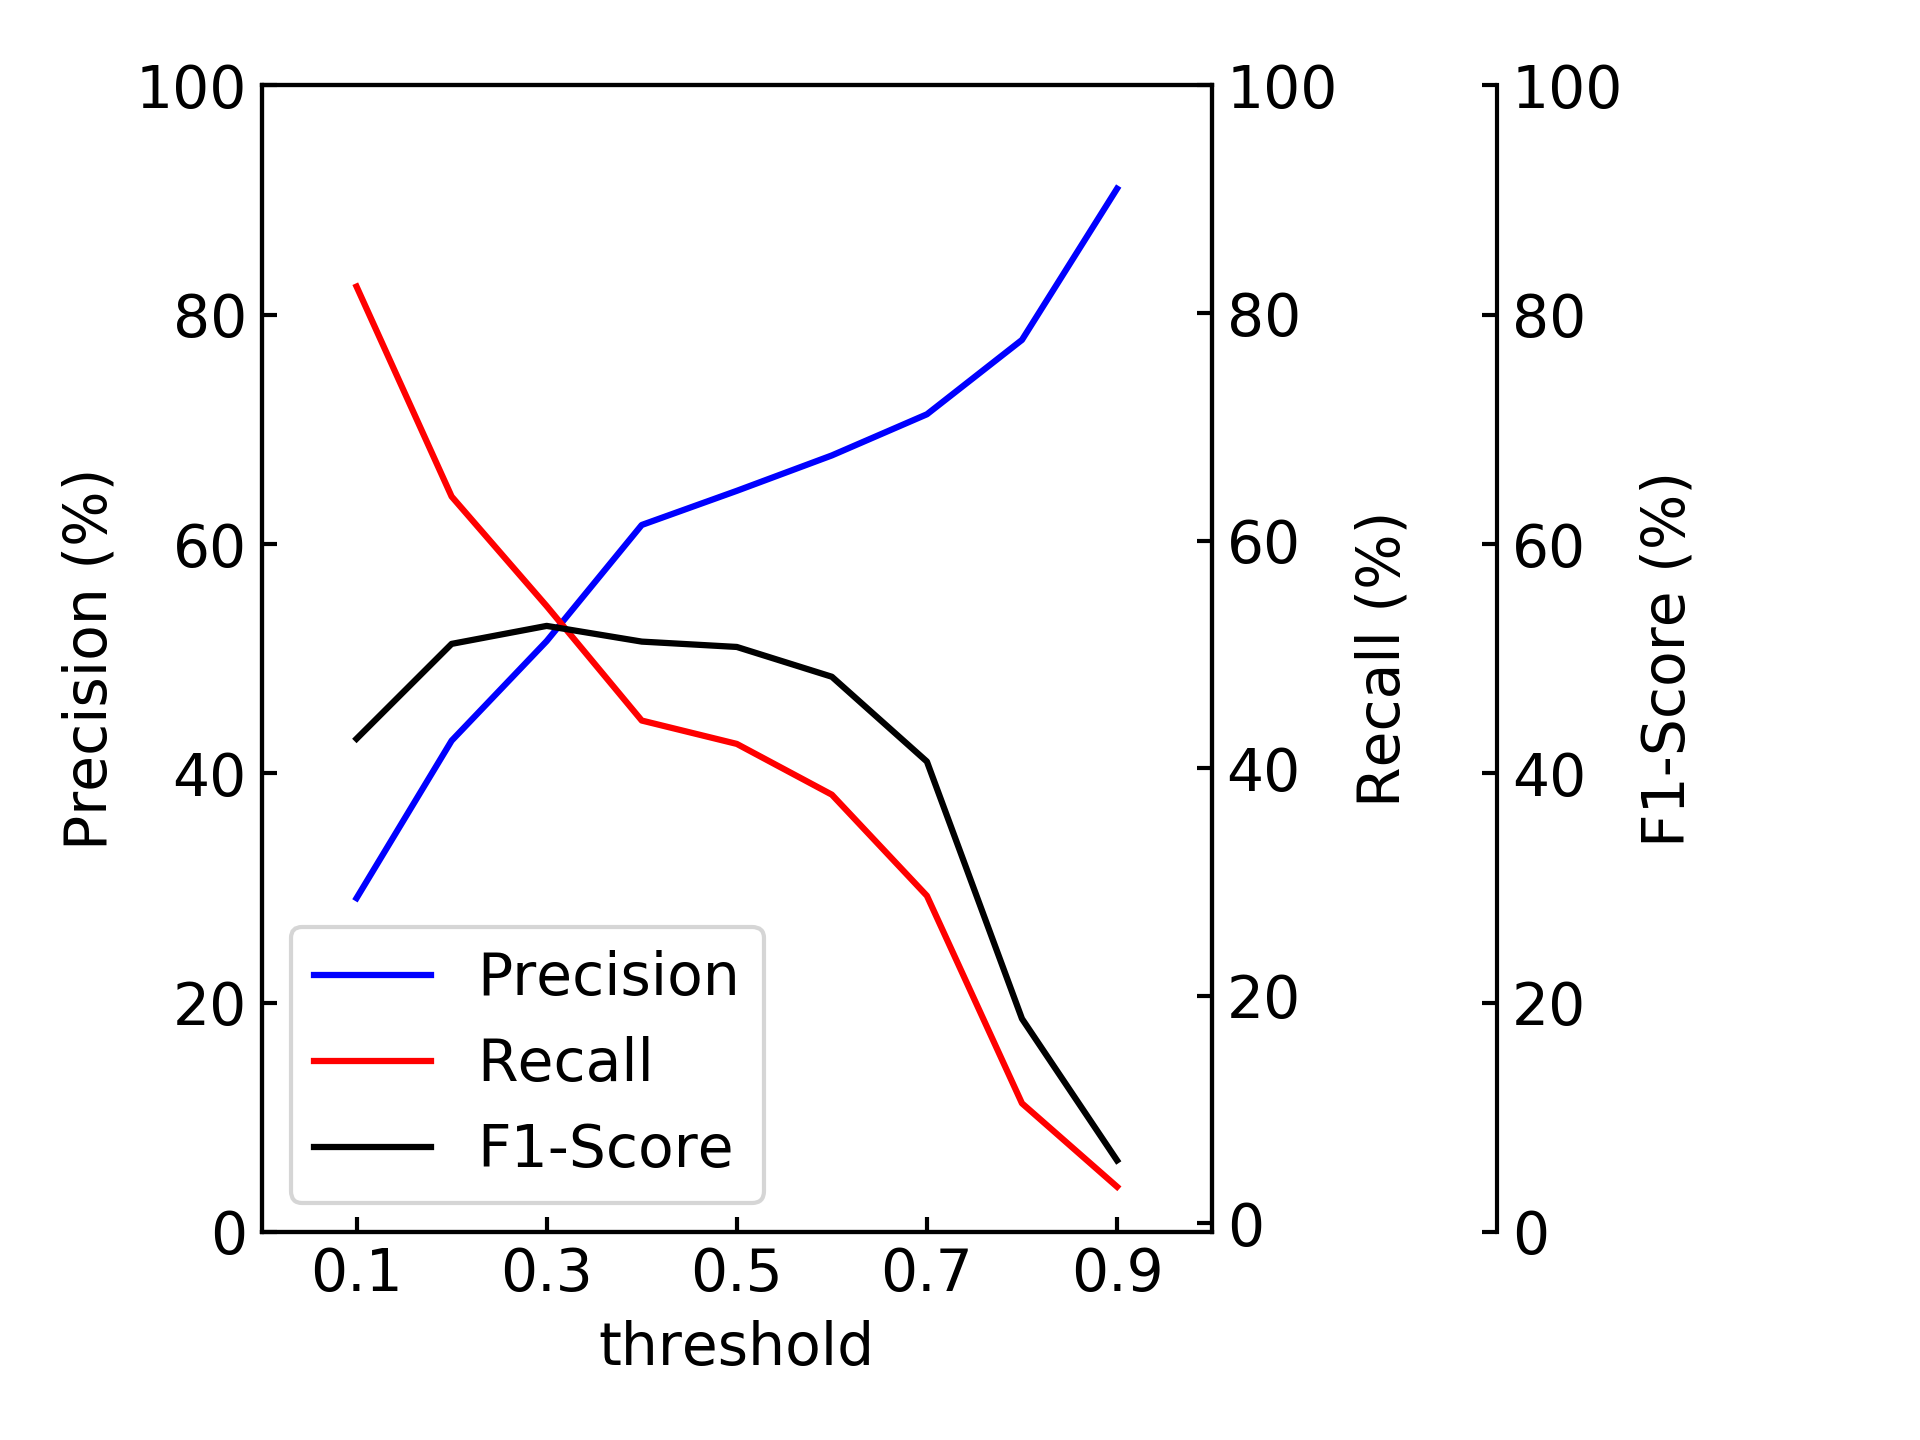
\includegraphics[width=150mm]{./fig/resnet3d_ethreshold.png}
        \caption{しきい値を変化させた際の適合率と再現率の変化}
        \label{figresnet3d_e_result_threshold}
    \end{center}
\end{figure}

\newpage
\subsection{モデル3の結果}
\begin{figure}[htbp]
    \begin{center}
        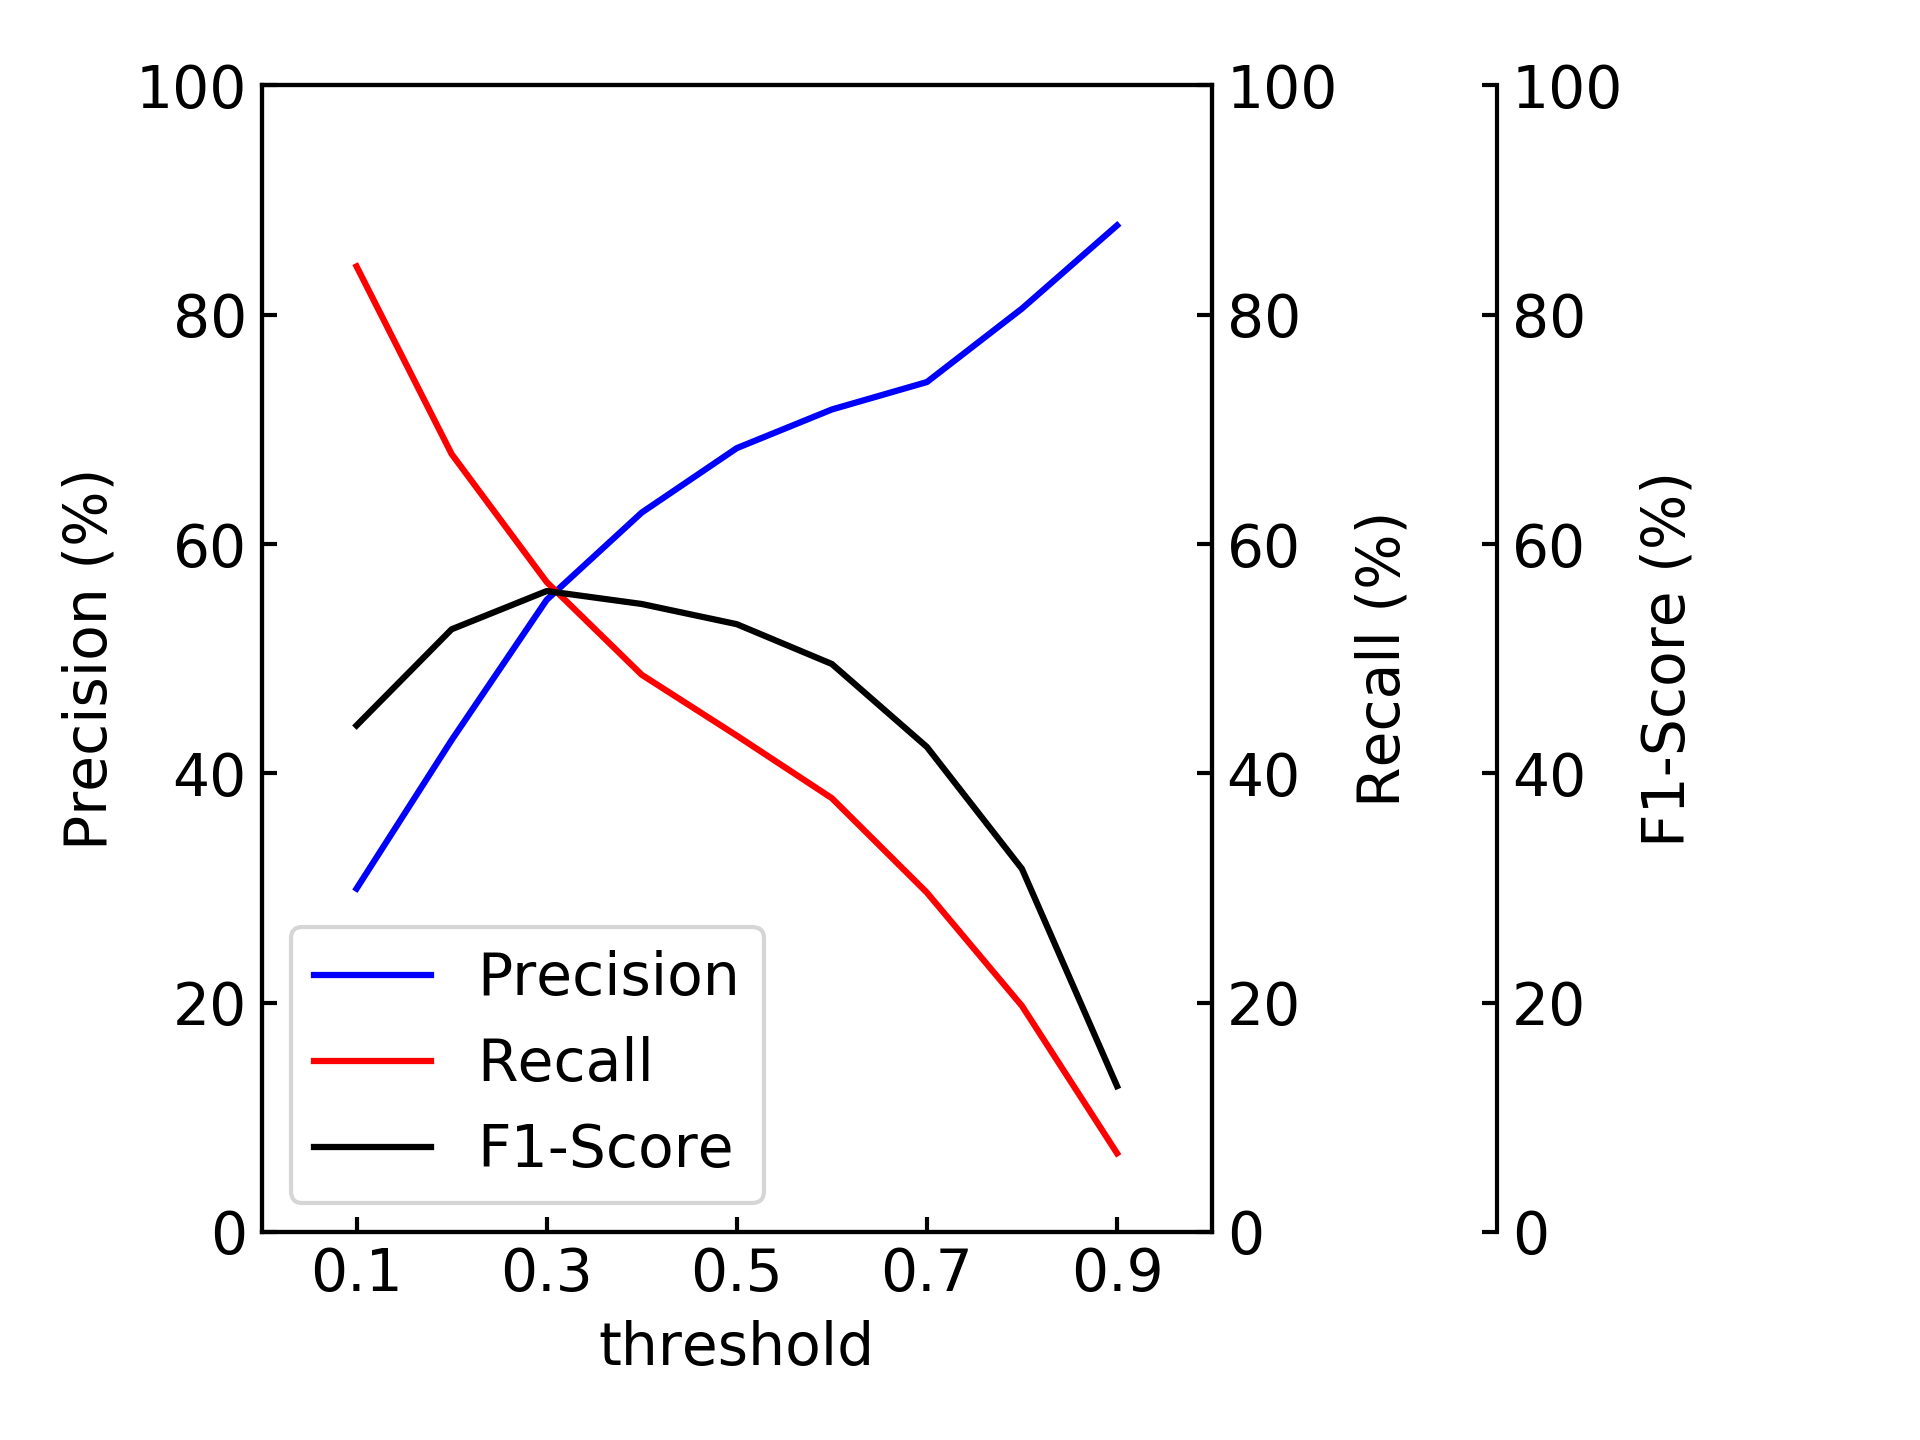
\includegraphics[width=150mm]{./fig/resnet3d_mthreshold.png}
        \caption{しきい値を変化させた際の適合率と再現率の変化}
        \label{fig:resnet3d_m_result_threshold}
    \end{center}
\end{figure}

\newpage
\subsection{モデル4の結果}
\begin{figure}[htbp]
    \begin{center}
        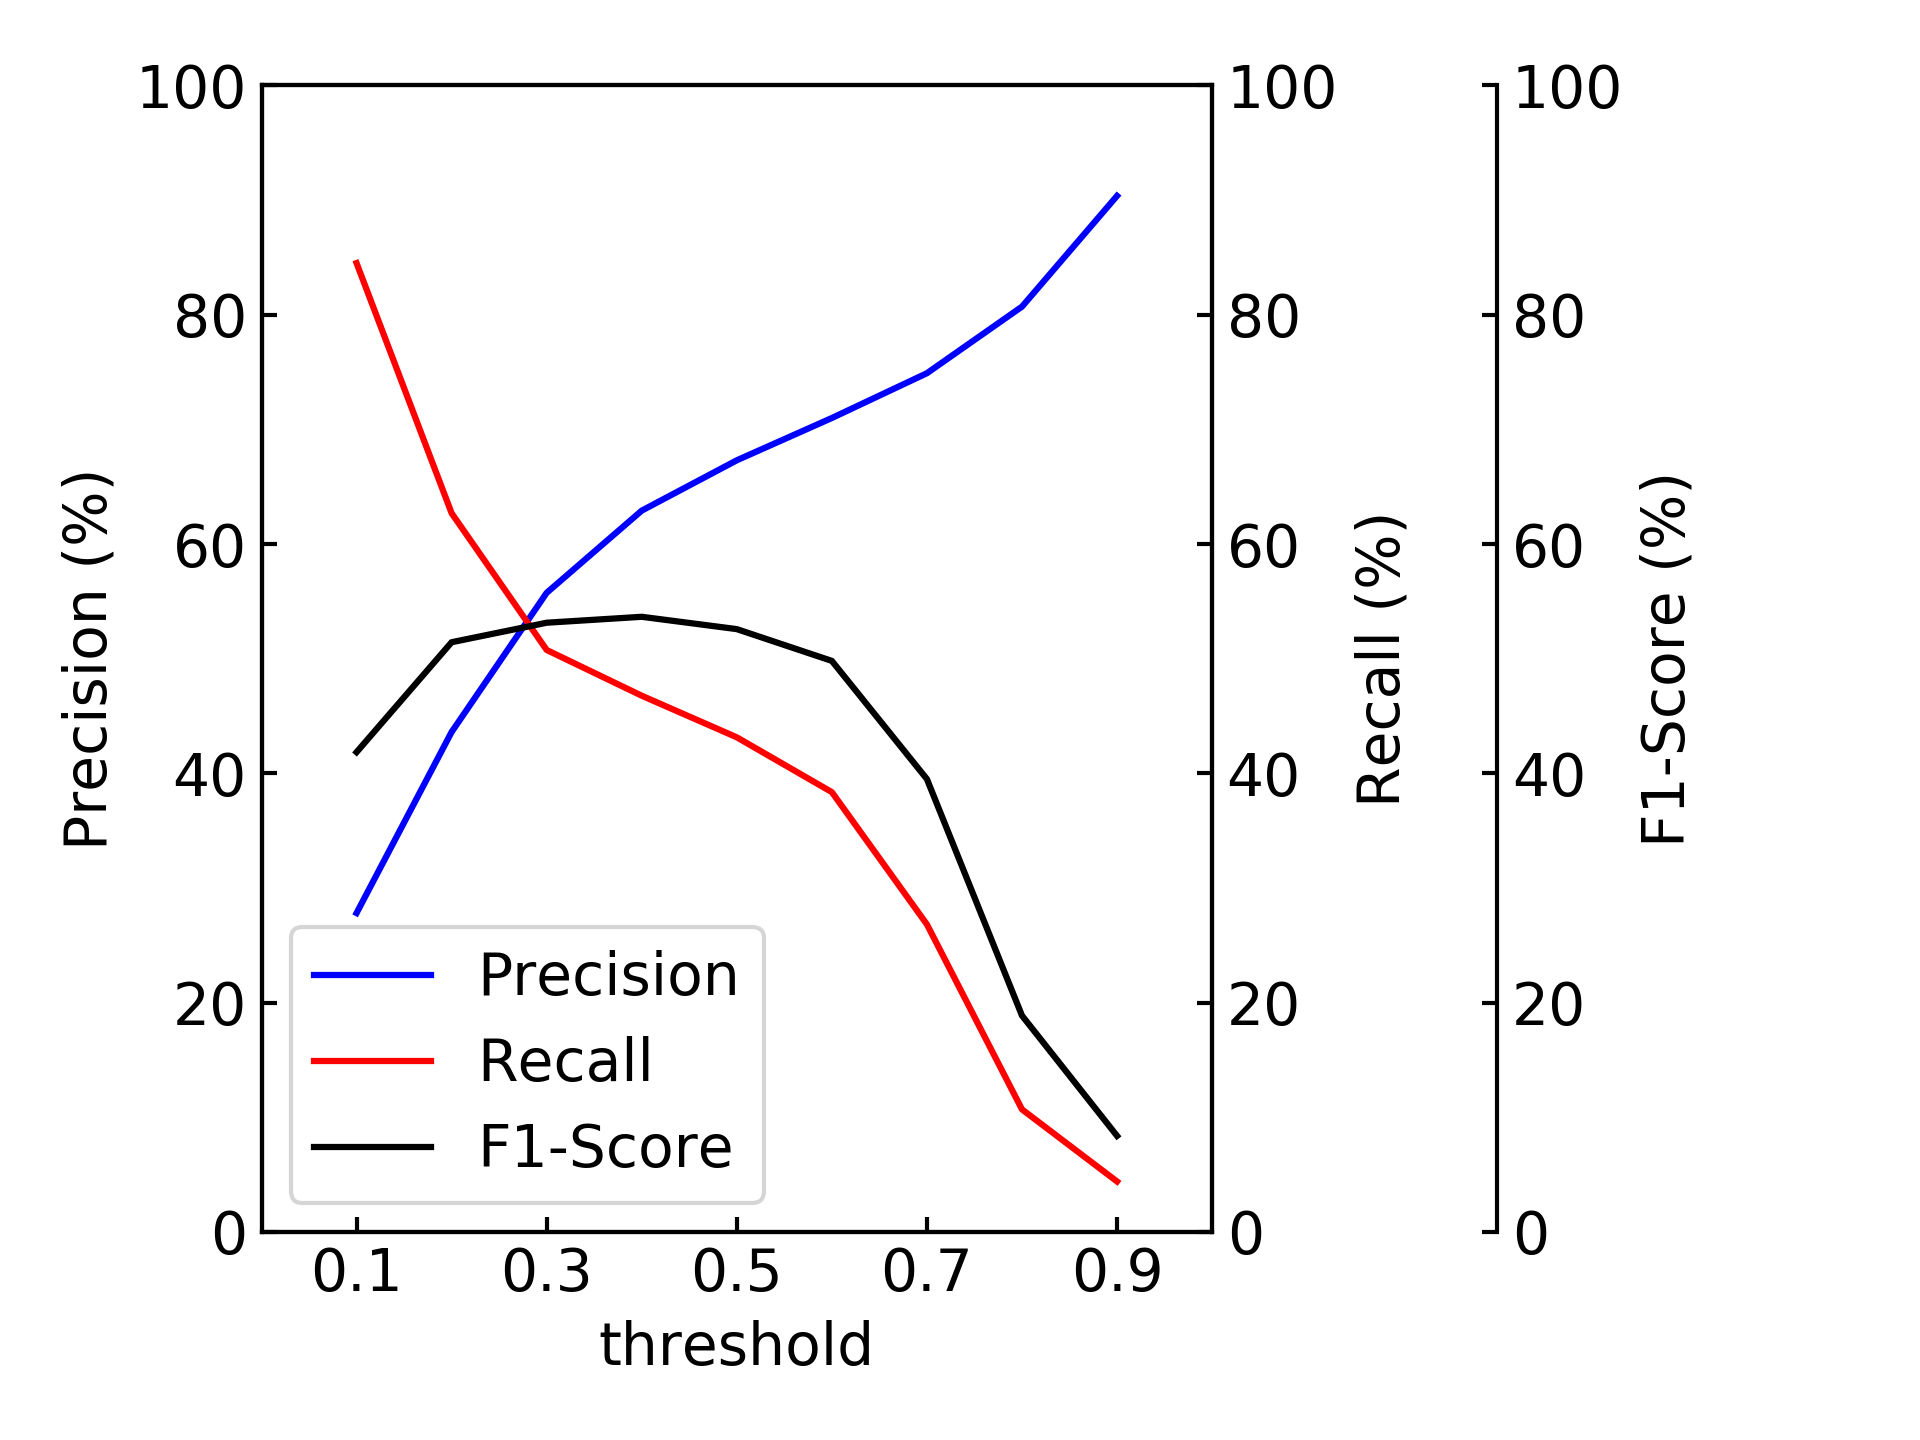
\includegraphics[width=150mm]{./fig/resnet3d_e_mthreshold.png}
        \caption{しきい値を変化させた際の適合率と再現率の変化}
        \label{fig:resnet3d_e_m_result_threshold}
    \end{center}
\end{figure}


\end{document}
